\documentclass{article}[12pt]

\usepackage[utf8]{inputenc}
\usepackage{amsfonts,amssymb,amsmath,subfigure}
\usepackage[pdftex]{graphicx}
\usepackage{epstopdf}
\usepackage{vmargin}
\usepackage{comment}
\usepackage{tikz,multicol}

\usepackage{algorithm}
\usepackage[noend]{algpseudocode}
\usepackage{tcolorbox}

\newtcolorbox{mybox}[3][]
{
  colframe = #2!25,
  colback  = #2!10,
  coltitle = #2!20!black,  
  title    = {#3},
  #1,
}


\newcommand*\Let[2]{\State #1 $\gets$ #2}
\algrenewcommand\algorithmicrequire{\textbf{Precondition:}}
\algrenewcommand\algorithmicensure{\textbf{Postcondition:}}




\excludecomment{solution}
%\includecomment{solution}

\title{IF111 - Algorithmes et structures de données\\EI5 - Algorithmes gloutons et arbres couvrants}
\date{\texttt{rfosse@labri.fr}}
\author{Rohan Fossé}
\begin{document}



\maketitle{}

\section*{Plus grande valeur}

On cherche à sélectionner cinq nombres de la liste suivante en cherchant à avoir leur somme la plus grande possible (maximiser une grandeur) et en s'interdisant de choisir deux nombres voisins (contrainte).\\

\begin{center}
  15 - 4 - 20 - 17 - 11 - 8 - 11 - 16 - 7 - 14 - 2 - 7 - 5 - 17 - 19 - 18 - 4 - 5 - 13 - 8\\  
\end{center}


Comme on souhaite avoir le plus grand résultat final, la stratégie gloutonne consiste à choisir à chaque étape le plus grand nombre possible dans les choix restants.
\begin{enumerate}
    \item Appliquez cet algorithme glouton sur le tableau;
    \item Vérifiez que {20,18,17,16,15} est une autre solution possible.
    \item Que dire de la solution gloutonne ?
\end{enumerate}

\section*{Problème du voyageur de commerce}

Un voyageur a ciblé plusieurs villes qu'il souhaite visiter. Il cherche un itinéraire passant par toutes ces villes et qui minimise la distance totale parcourue. Les villes peuvent être visitées dans n'importe quel ordre mais aucune ne doit être négligée, et le visiteur doit revenir à la fin à sa ville de départ.\\

Le voyageur part de Nancy et souhaite visiter Metz, Paris, Reims et Troyes, avant de retourner à Nancy.\\

Voici un tableau donnant les distances kilométriques entre chacune des ces villes.

\begin{figure}[h!]
    \centering
    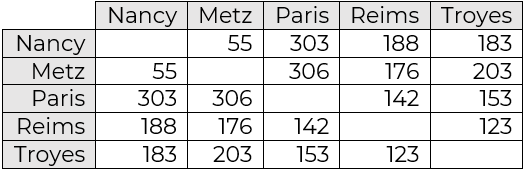
\includegraphics[scale=0.7]{tableau_voyageur.png}
    \label{fig:my_label}
\end{figure}

\begin{enumerate}
    \item Quelle est la stratégie gloutonne à mettre en oeuvre ?
    \item Mettez en oeuvre cette stratégie et donnez la solution.
    \item  Calculez la distance totale pour le parcours Metz - Reims - Paris - Troyes (départ et arrivée à Nancy sous-entendus)
    \item Que dire de la solution gloutonne ?
\end{enumerate}
    
\section*{Le parc d'attraction}
    
Vous visitez un parc d'attractions proposant des spectacles à différents horaires. Voici les horaires des différents spectacles :

\begin{table}[h!]
\begin{tabular}{|c|c|c|c|c|c|c|c}
\hline
\textbf{spectacle} & \textbf{A} & \textbf{B}  & \textbf{C} & \textbf{D} & \textbf{E} & \textbf{F} & \textbf{G} \\ \hline
\textbf{horaire}   & 10h-11h    & 10h30-11h30 & 11h-12h30  & 11h30-12h  & 12h-13h    & 13h-15h    & 13h30-14h  \\ \hline
\end{tabular}
\end{table}

\begin{table}[h!]
\centering
\begin{tabular}{l|l|l|}
\hline
\textbf{H} & \textbf{I} & \textbf{J} \\ \hline
14h-15h30  & 15h-16h    & 16h-17h30  \\ \hline
\end{tabular}
\end{table}

Vous avez remarqué qu'il n'est pas possible d'assister à tous les spectacles puisque certains ont lieu à des moments communs. Vous souhaitez assister à un maximum de spectacles sur la journée. Quels spectacles devez-vous choisir ?

    \begin{enumerate}
        \item Trouvez deux algorithmes gloutons pour ce problème
        \item Appliquez ces deux stratégies au problème.
        \item Laquelle donne la meilleure solution ?
    \end{enumerate}
    
    
\section*{La clé USB}

Nous disposons d’une clé USB qui est déjà bien remplie et sur laquelle il ne reste que 5 Go de libre. Nous souhaitons copier sur cette clé des fichiers vidéos pour l’emporter en voyage. Chaque fichier a un poids et chaque vidéo a une durée. La durée n’est pas proportionnelle à la taille car les fichiers sont de format différents, certaines vidéos sont de grande qualité, d’autres sont très compressées. Le tableau qui suit présente les 7 fichiers disponibles avec les durées données en minutes.

\begin{table}[h!]
\centering
\begin{tabular}{|c|c|c|}
\hline
\multicolumn{1}{|c|}{\textbf{Nom}} & \multicolumn{1}{c|}{\textbf{Durée en min (valeur)}} & \multicolumn{1}{c|}{\textbf{Poids}} \\ \hline
Vidéo A                            & 114                                                 & 4.57 Go                             \\ \hline
Vidéo B                            & \multicolumn{1}{c|}{32}                             & 630 Mo                              \\ \hline
Vidéo C                            & 20                                                  & 1.65 Go                             \\ \hline
Vidéo D                            & 4                                                   & 85 Mo                               \\ \hline
Vidéo E                            & 18                                                  & 2,15 Go                             \\ \hline
Vidéo F                            & 80                                                  & 2,71 Go                             \\ \hline
Vidéo G                            & 5                                                   & 320 Mo                              \\ \hline
\end{tabular}
\end{table}

Quelles vidéos copier sur la clé USB pour que la durée des vidéos soient la plus grande possible tout en ne dépassant pas 5 Go ? Donner l'algorithme glouton.

\section*{Bipartition}
Étant donné un ensemble de n nombres, répartissez les en 2 sous-ensembles tels que la somme des éléments du premier soit égal à la somme des éléments du second. Proposez des algorithmes gloutons pour résoudre ce problème. Appliquez les aux ensembles suivants :
\begin{center}
   \{2, 10, 3, 8, 5, 7, 9, 5, 3, 2\}\\
\{771, 121, 281, 854, 885, 734, 486, 1003, 83, 62\} 
\end{center}

\section*{Arbres non-isomorphes}
Donner tous les arbres non-isomorphes à :
\begin{enumerate}
    \item 1, 2 ou 3 sommets
    \item 4 sommets
    \item 5 sommets
\end{enumerate}

\section*{Arbres couvrants}

Soit G = (S, A) un graphe non orienté (pas forcément connexe). on appelle forêt couvrante maximale tout sous-graphe de G couvrant, sans cycle, et telle que l'ajout d'une arête quelconque crée un cycle.

\begin{enumerate}
    \item Montrer que si G est connexe, toute forêt couvrante maximale est un arbre couvrant.
    \item Montrer que si le nombre d'arêtes d'une forêt couvrante est $|S|$ - k où k est le nombre de composantes connexes de G.
\end{enumerate}

\section*{Algorithme de Prim}

Appliquer l'algorithme de Prim pour trouver un arbre couvrant de poids minimum du graphe G représenté sur la figure ci-dessous.

\begin{figure}[h!]
    \centering
    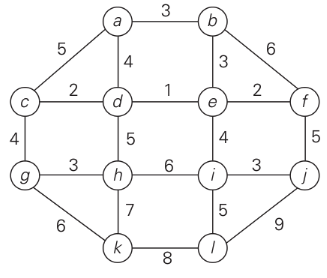
\includegraphics[scale=0.8]{Prim-1.png}
    \label{fig:my_label}
\end{figure}

\section*{Algorithme de Kruskal et Prim}

On considère le graphe non orienté valué G suivant: 

\begin{figure}[h!]
    \centering
    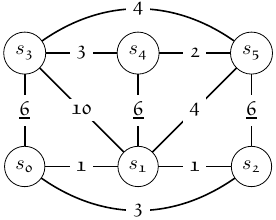
\includegraphics{Kruskal-1.png}
    \label{fig:my_label}
\end{figure}


 Déterminer un arbre recouvrant de G de poids minimum depuis le sommet $s_0$ en utilisant l'algorithme de Kruskal. Déterminer l'arbre couvrant de G en utilisant l'algorithme de Pri
 
 \newpage
\section*{Algorithme de Kruskal}
En détaillant toutes les  étapes, appliquez l’algorithme de Kruskal sur le graphe
suivant.

\begin{figure}[h!]
    \centering
    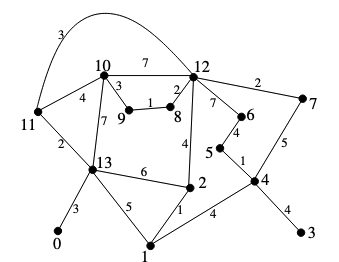
\includegraphics[scale=0.6]{Kruskal-2.png}
    \label{fig:my_label}
\end{figure}

Quel est le poids d’un arbre couvrant de poids minimal ?\\
En utilisant le même graphe que la question précédente, déterminer comment calculer le poids d’un arbre
couvrant de poids maximum. Donner un arbre de poids couvrant maximal.



\end{document}